% =====================================================================
%  SECTION 5 -- THEORETICAL MODEL  (rewritten, self-contained)
%  Coupled magnetic-mechanical oscillator: two copper leaf springs with
%  repelling magnets.
%  Build:  tectonic -X compile theory_section.tex   (or pdflatex x2)
%  Needs fig_release.pdf in the same folder (made by plot in theory_guide).
% =====================================================================
\documentclass[11pt,a4paper]{article}
\usepackage[a4paper,margin=2.4cm]{geometry}
\usepackage[T1]{fontenc}
\usepackage[utf8]{inputenc}
\usepackage{lmodern}
\usepackage{amsmath,amssymb,bm}
\usepackage{booktabs,array}
\usepackage{enumitem}
\usepackage{xcolor}
\usepackage{graphicx}
\usepackage{tikz}
\usetikzlibrary{decorations.pathmorphing,arrows.meta,calc,positioning,patterns}
\usepackage{pgfplots}
\pgfplotsset{compat=1.18}
\usepackage{caption}
\captionsetup{font=small,labelfont=bf,width=0.92\textwidth}
\usepackage{tcolorbox}
\usepackage{float}

% ---- house style shared with the rest of the essay (Section 1 figures) ----
\colorlet{copper}{orange!80!black}      % leaf springs
\colorlet{clampgray}{gray!60}           % clamps
\colorlet{basegray}{gray!30}            % non-magnetic base
\colorlet{magnetS}{red!70}              % S pole (red)   -- as in Fig. 1 of the essay
\colorlet{magnetN}{blue!70}             % N pole (blue)
% \magnetSN{x}{y}{width}{height} / \magnetNS{...}: two-colour magnet block with its lower-left
%   corner at (x,y); SN / NS is the pole order from left to right (S = red, N = blue, as in
%   Figure 1 of the essay). Pole letters are printed in white.
\newcommand{\magnetSN}[4]{%
  \fill[magnetS] (#1,#2) rectangle ({#1+#3/2},{#2+#4});
  \fill[magnetN] ({#1+#3/2},#2) rectangle ({#1+#3},{#2+#4});
  \node[white,font=\tiny] at ({#1+#3/4},{#2+#4/2}) {S};
  \node[white,font=\tiny] at ({#1+3*#3/4},{#2+#4/2}) {N};}
\newcommand{\magnetNS}[4]{%
  \fill[magnetN] (#1,#2) rectangle ({#1+#3/2},{#2+#4});
  \fill[magnetS] ({#1+#3/2},#2) rectangle ({#1+#3},{#2+#4});
  \node[white,font=\tiny] at ({#1+#3/4},{#2+#4/2}) {N};
  \node[white,font=\tiny] at ({#1+3*#3/4},{#2+#4/2}) {S};}
\newcommand{\muz}{\mu_0}
\newcommand{\mum}{\mu_{\mathrm m}}
\newcommand{\dd}{\mathrm{d}}
\newcommand{\un}[1]{\,\mathrm{#1}}
\newtcolorbox{keybox}{colback=blue!4,colframe=blue!50!black,boxrule=0.6pt,arc=2pt,left=4pt,right=4pt,top=3pt,bottom=3pt}
\newtcolorbox{notebox}{colback=gray!6,colframe=gray!55!black,boxrule=0.5pt,arc=2pt,left=4pt,right=4pt,top=3pt,bottom=3pt,fontupper=\small}



\begin{document}
\section*{Figures of Section 5 (theory) --- source collection}
\noindent Each figure below is the same TikZ/pgfplots code as in \texttt{theory\_section.tex}; copy the corresponding \verb|\begin{figure}...\end{figure}| block (and the colour/magnet definitions from the preamble of this file). Figure~13 is the external file \texttt{fig\_release.pdf}, produced by \texttt{make\_fig\_release.py}. House style: springs \texttt{copper} (= \texttt{orange!80!black}), clamps \texttt{gray!60}, base \texttt{gray!30}, magnets S = \texttt{red!70}, N = \texttt{blue!70}, exactly as in the setup figure of Section~1.
\bigskip

\begin{figure}[H]
\centering
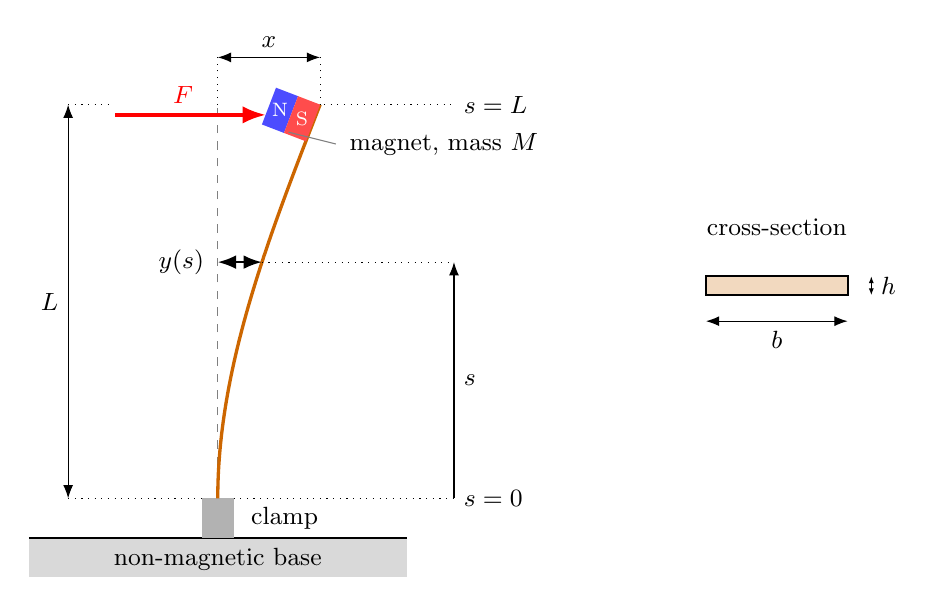
\begin{tikzpicture}[scale=1,>=Latex]
% base and clamp (style of Section 1)
\fill[basegray] (-2.4,-0.5) rectangle (2.4,0);  \draw[thick] (-2.4,0)--(2.4,0);
\node[font=\small] at (0,-0.27) {non-magnetic base};
\fill[clampgray] (-0.2,0) rectangle (0.2,0.5);
\node[font=\small,anchor=west] at (0.3,0.25) {clamp};
% undeflected (dashed) and deflected strip: y = x s^2(3L-s)/(2L^3), L = 5
\draw[dashed,gray] (0,0.5)--(0,5.5);
\draw[very thick,copper,domain=0:5,samples=50,variable=\s] plot ({1.3*\s*\s*(15-\s)/250},{0.5+\s});
% magnet glued to the LEFT face of the strip at the tip (frame tilted with the strip, 21 deg);
% N pole outwards (towards the other magnet), S pole against the strip -- as spring 2 in the setup figure
\begin{scope}[shift={(1.3,5.5)},rotate=-21]
  \fill[magnetN] (-0.6,-0.5) rectangle (-0.3,0.0);
  \fill[magnetS] (-0.3,-0.5) rectangle (0.0,0.0);
  \node[white,font=\scriptsize] at (-0.45,-0.25){N}; \node[white,font=\scriptsize] at (-0.15,-0.25){S};
\end{scope}
\node[font=\small,anchor=west] at (1.55,5.0) {magnet, mass $M$};
\draw[gray,thin] (0.9,5.15)--(1.5,5.0);
% tip force: horizontal, through the centre of the magnet, arrow head touching its outer face
\draw[->,red,very thick] (-1.3,5.37)--(0.61,5.37) node[pos=0.45,above,font=\small]{$F$};
% tip deflection
\draw[<->] (0,6.1)--(1.3,6.1) node[midway,above,font=\small]{$x$};
\draw[dotted] (0,5.5)--(0,6.1); \draw[dotted] (1.3,5.5)--(1.3,6.1);
% free length L
\draw[<->] (-1.9,0.5)--(-1.9,5.5) node[midway,left,font=\small]{$L$};
\draw[dotted] (-1.9,0.5)--(-0.2,0.5); \draw[dotted] (-1.9,5.5)--(-1.35,5.5);
% coordinate s and deflection y(s) at a general point (s = 3: phi = 0.432)
\draw[<->,thick] (0,3.5)--(0.56,3.5); \node[font=\small,anchor=east] at (-0.05,3.5){$y(s)$};
\draw[dotted] (0.56,3.5)--(3.0,3.5);
\draw[->] (3.0,0.5)--(3.0,3.5) node[midway,right,font=\small]{$s$};
\draw[dotted] (0.2,0.5)--(3.0,0.5);
\node[font=\small,anchor=west] at (3.0,0.5){$s=0$};
\draw[dotted] (1.35,5.5)--(3.0,5.5); \node[font=\small,anchor=west] at (3.0,5.5){$s=L$};
% cross-section inset
\begin{scope}[shift={(6.2,3.2)}]
\node[font=\small] at (0.9,0.75) {cross-section};
\draw[thick,fill=copper!25] (0,-0.12) rectangle (1.8,0.12);
\draw[<->] (0,-0.45)--(1.8,-0.45) node[midway,below,font=\small]{$b$};
\draw[{Latex[length=2.5pt]}-{Latex[length=2.5pt]}] (2.1,-0.12) -- (2.1,0.12)
  node[midway, right, font=\small]{$h$};
\end{scope}
\end{tikzpicture}
\caption{Geometry of the leaf spring.}
\end{figure}

\begin{figure}[H]
\centering
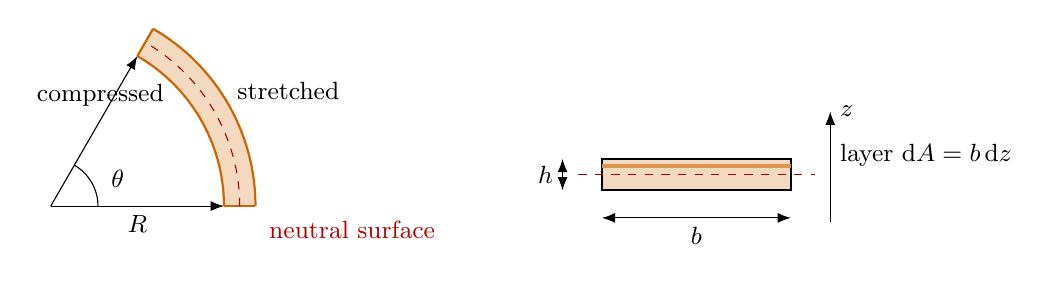
\begin{tikzpicture}[scale=1,>=Latex]
% bent element of the strip
\fill[copper!25] (2.2,0) arc (0:60:2.2) -- ({2.6*cos(60)},{2.6*sin(60)}) arc (60:0:2.6) -- cycle;
\draw[thick,copper] (2.2,0) arc (0:60:2.2);
\draw[thick,copper] (2.6,0) arc (0:60:2.6);
\draw[thick,copper] (2.2,0)--(2.6,0);
\draw[thick,copper] ({2.2*cos(60)},{2.2*sin(60)})--({2.6*cos(60)},{2.6*sin(60)});
\draw[dashed,red!70!black] (2.4,0) arc (0:60:2.4);
\node[red!70!black,anchor=west,font=\small] at (2.65,-0.3) {neutral surface};
\draw[->] (0,0)--(2.2,0) node[midway,below,font=\small]{$R$};
\draw[->] (0,0)--({2.2*cos(60)},{2.2*sin(60)});
\draw (0.6,0) arc (0:60:0.6); \node[font=\small] at (0.85,0.35) {$\theta$};
\node[anchor=west,font=\small] at ({2.65*cos(32)},{2.75*sin(32)}) {stretched};
\node[anchor=east,font=\small] at ({2.1*cos(42)},{2.1*sin(42)}) {compressed};
% cross-section with z
\begin{scope}[shift={(7.0,0.4)}]
\draw[thick,fill=copper!25] (0,-0.2) rectangle (2.4,0.2);
\draw[dashed,red!70!black] (-0.3,0)--(2.7,0);
\fill[copper!70] (0,0.08) rectangle (2.4,0.14);
\draw[->] (2.9,-0.6)--(2.9,0.8) node[right,font=\small]{$z$};
\draw[<->] (-0.5,-0.2)--(-0.5,0.2) node[midway,left,font=\small]{$h$};
\draw[<->] (0,-0.55)--(2.4,-0.55) node[midway,below,font=\small]{$b$};
\node[right,font=\small] at (2.9,0.25) {layer $\dd A=b\,\dd z$};
\end{scope}
\end{tikzpicture}
\caption{Left: a short element of the strip bent to radius of curvature $R$ through angle $\theta$. Layers outside the neutral surface (dashed) are stretched, layers inside are compressed, by a strain $z/R$. Right: the cross-section, with $z$ measured from the neutral surface; a layer of area $\dd A=b\,\dd z$ at height $z$ carries stress $Ez/R$, and the sum of their moments is $EI/R$.}
\end{figure}

\begin{figure}[H]
\centering
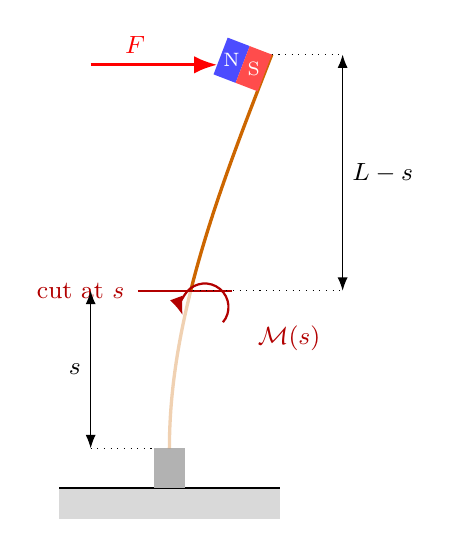
\begin{tikzpicture}[scale=1,>=Latex]
\fill[basegray] (-1.4,-0.4) rectangle (1.4,0); \draw[thick] (-1.4,0)--(1.4,0);
\fill[clampgray] (-0.2,0) rectangle (0.2,0.5);
% strip: part below the cut faint, part above the cut full colour
\draw[very thick,copper,opacity=0.3,domain=0:2,samples=30,variable=\t] plot ({1.3*\t*\t*(15-\t)/250},{0.5+\t});
\draw[very thick,copper,domain=2:5,samples=40,variable=\t] plot ({1.3*\t*\t*(15-\t)/250},{0.5+\t});
% magnet on the left face at the tip, as in Figure 1
\begin{scope}[shift={(1.3,5.5)},rotate=-21]
  \fill[magnetN] (-0.6,-0.5) rectangle (-0.3,0.0);
  \fill[magnetS] (-0.3,-0.5) rectangle (0.0,0.0);
  \node[white,font=\scriptsize] at (-0.45,-0.25){N}; \node[white,font=\scriptsize] at (-0.15,-0.25){S};
\end{scope}
% cut
\draw[thick,red!70!black] (-0.4,2.5)--(0.8,2.5);
\node[red!70!black,anchor=east,font=\small] at (-0.45,2.5) {cut at $s$};
% tip force, arrow head touching the magnet
\draw[->,red,very thick] (-1.0,5.37)--(0.61,5.37) node[pos=0.35,above,font=\small]{$F$};
% lever arm
\draw[<->] (2.2,2.5)--(2.2,5.5) node[midway,right,font=\small]{$L-s$};
\draw[dotted] (0.3,2.5)--(2.2,2.5); \draw[dotted] (1.3,5.5)--(2.2,5.5);
% s
\draw[<->] (-1.0,0.5)--(-1.0,2.5) node[midway,left,font=\small]{$s$};
\draw[dotted] (-1.0,0.5)--(-0.2,0.5);
% internal moment at the cut
\draw[->,thick,red!70!black] (0.68,2.1) arc (-40:200:0.3);
\node[red!70!black,anchor=west,font=\small] at (1.0,1.9) {$\mathcal M(s)$};
\end{tikzpicture}
\caption{Finding the bending moment. The part of the strip above an imaginary cut at height $s$ (full colour, together with the magnet) is acted on by the tip force $F$, with lever arm $L-s$, and by the internal moment $\mathcal M(s)$ exerted on it by the part below the cut (faint). For equilibrium of the upper part, $\mathcal M(s)=F(L-s)$: largest at the clamp, zero at the tip.}
\end{figure}

\begin{figure}[H]
\centering
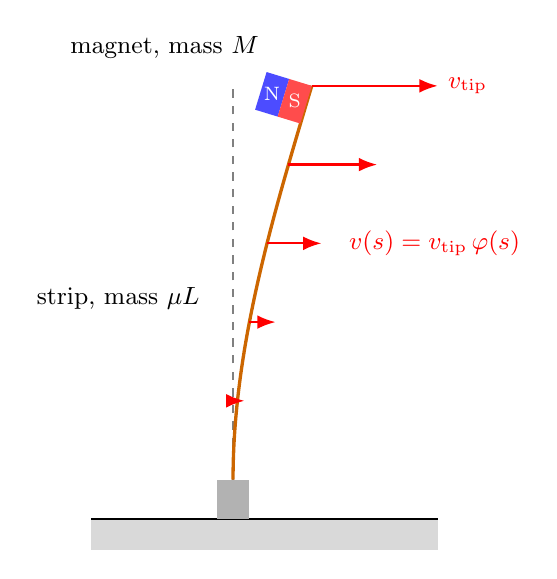
\begin{tikzpicture}[scale=1,>=Latex]
\fill[basegray] (-1.8,-0.4) rectangle (2.6,0); \draw[thick] (-1.8,0)--(2.6,0);
\fill[clampgray] (-0.2,0) rectangle (0.2,0.5);
\draw[dashed,gray] (0,0.5)--(0,5.5);
\draw[very thick,copper,domain=0:5,samples=50,variable=\t] plot ({1.0*\t*\t*(15-\t)/250},{0.5+\t});
% velocity arrows, length proportional to phi(s)
\foreach \t in {1,2,3,4}{
  \pgfmathsetmacro{\v}{1.6*\t*\t*(15-\t)/250}
  \draw[->,red,thick] ({1.0*\t*\t*(15-\t)/250},{0.5+\t}) -- ++({\v},0);
}
% magnet on the left face at the tip (local slope about 17 deg)
\begin{scope}[shift={(1.0,5.5)},rotate=-17]
  \fill[magnetN] (-0.6,-0.5) rectangle (-0.3,0.0);
  \fill[magnetS] (-0.3,-0.5) rectangle (0.0,0.0);
  \node[white,font=\scriptsize] at (-0.45,-0.25){N}; \node[white,font=\scriptsize] at (-0.15,-0.25){S};
\end{scope}
\node[font=\small,anchor=south east] at (0.45,5.72) {magnet, mass $M$};
% tip velocity (magnet and strip tip move together)
\draw[->,red,thick] (1.0,5.5) -- ++(1.6,0) node[right,font=\small]{$v_{\rm tip}$};
\node[red,anchor=west,font=\small] at (1.35,3.5) {$v(s)=v_{\rm tip}\,\varphi(s)$};
\node[font=\small,anchor=east] at (-0.3,2.8) {strip, mass $\mu L$};
\end{tikzpicture}
\caption{Rayleigh's method. During the oscillation every point of the strip is assumed to move in proportion to the static deflection curve $\varphi(s)$ of equation~(9), so its velocity is $v_{\rm tip}\varphi(s)$: nearly zero near the clamp, equal to the magnet's velocity at the tip (arrows). The strip's kinetic energy is the same as that of a point mass $\tfrac{33}{140}\mu L$ moving with the tip.}
\end{figure}

\begin{figure}[H]
\centering
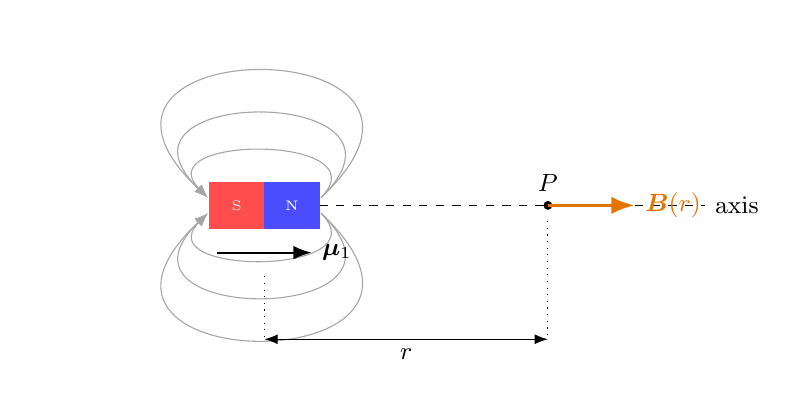
\begin{tikzpicture}[scale=1,>=Latex]
\foreach \r in {1.0,1.7,2.5}{
  \draw[gray!70,->] (0.72,0.1) .. controls (\r+0.5,\r*0.9) and (-\r-0.5,\r*0.9) .. (-0.72,0.1);
  \draw[gray!70,->] (0.72,-0.1) .. controls (\r+0.5,-\r*0.9) and (-\r-0.5,-\r*0.9) .. (-0.72,-0.1);
}
\magnetSN{-0.7}{-0.3}{1.4}{0.6}
\draw[->,thick] (-0.6,-0.6)--(0.6,-0.6) node[right,font=\small]{$\bm\mu_1$};
\draw[dashed] (0.7,0)--(5.6,0) node[right,font=\small]{axis};
\fill (3.6,0) circle (1.6pt); \node[above,font=\small] at (3.6,0.05){$P$};
\draw[->,very thick,orange!90!black] (3.6,0)--(4.7,0) node[right,font=\small]{$\bm B(r)$};
\draw[<->] (0,-1.7)--(3.6,-1.7) node[midway,below,font=\small]{$r$};
\draw[dotted] (0,-0.9)--(0,-1.7); \draw[dotted] (3.6,-0.2)--(3.6,-1.7);
\end{tikzpicture}
\caption{The field of a small magnet (a magnetic dipole of moment $\bm\mu_1$, magnitude $\mum$, pointing from S to N). Grey: field lines. At a point $P$ on the axis, at distance $r$ from the \emph{centre} of the magnet, the field points along the axis in the direction of the moment, with magnitude $\muz2\mum/4\pi r^3$.}
\end{figure}

\begin{figure}[H]
\centering
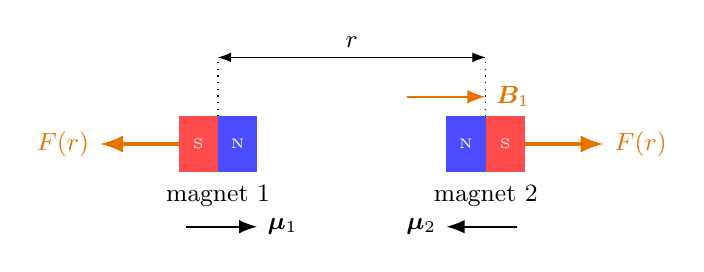
\begin{tikzpicture}[scale=1,>=Latex]
\magnetSN{0}{-0.35}{1.0}{0.7}
\magnetNS{3.4}{-0.35}{1.0}{0.7}
\node[font=\small,below] at (0.5,-0.4){magnet 1}; \node[font=\small,below] at (3.9,-0.4){magnet 2};
\draw[->,thick] (0.1,-1.05)--(1.0,-1.05) node[right,font=\small]{$\bm\mu_1$};
\draw[->,thick] (4.3,-1.05)--(3.4,-1.05) node[left,font=\small]{$\bm\mu_2$};
\draw[->,thick,orange!90!black] (2.9,0.6)--(3.9,0.6) node[right,font=\small]{$\bm B_1$};
\draw[<->] (0.5,1.1)--(3.9,1.1) node[midway,above,font=\small]{$r$};
\draw[dotted] (0.5,0.35)--(0.5,1.1); \draw[dotted] (3.9,0.35)--(3.9,1.1);
\draw[->,very thick,orange!90!black] (4.4,0)--(5.4,0) node[right,font=\small]{$F(r)$};
\draw[->,very thick,orange!90!black] (0,0)--(-1.0,0) node[left,font=\small]{$F(r)$};
\end{tikzpicture}
\caption{Two identical magnets on a common axis with like poles (N) facing. The field $\bm B_1$ of magnet~1 at magnet~2 points to the right; the moment $\bm\mu_2$ of magnet~2 points to the left, so the energy $-\bm\mu_2\cdot\bm B_1$ is positive and decreases with $r$: the magnets repel with $F(r)=3\muz\mum^2/2\pi r^4$, equal and opposite on the two magnets.}
\end{figure}

\begin{figure}[H]
\centering
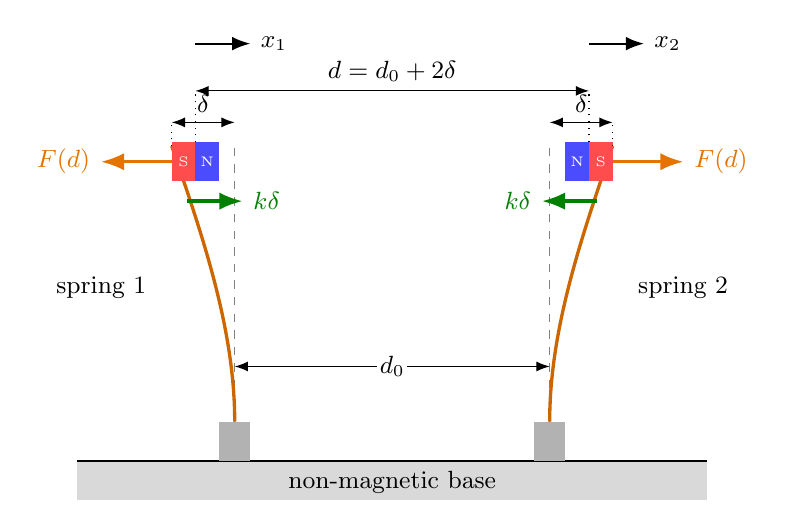
\begin{tikzpicture}[scale=1,>=Latex]
\fill[basegray] (-4.0,-0.5) rectangle (4.0,0); \draw[thick] (-4.0,0)--(4.0,0);
\node[font=\small] at (0,-0.27) {non-magnetic base};
\foreach \sx in {-1,1}{
  \fill[clampgray] ({\sx*2.0-0.2},0) rectangle ({\sx*2.0+0.2},0.5);
  \draw[dashed,gray] ({\sx*2.0},0.5)--({\sx*2.0},4.0);
  \draw[very thick,copper,domain=0:3.5,samples=40,variable=\s]
        plot ({\sx*2.0+\sx*0.8*\s*\s*(10.5-\s)/85.75},{0.5+\s});
}
% magnets glued to the inner faces of the strips (tips at x = -2.8 and +2.8), N poles facing
\magnetSN{-2.8}{3.55}{0.6}{0.5}
\magnetNS{2.2}{3.55}{0.6}{0.5}
\node[font=\small,anchor=east] at (-3.0,2.2) {spring 1}; \node[font=\small,anchor=west] at (3.0,2.2) {spring 2};
% clamp spacing and centre-to-centre separation
\draw[<->] (-2.0,1.2)--(2.0,1.2) node[midway,fill=white,inner sep=1pt,font=\small]{$d_0$};
\draw[<->] (-2.5,4.7)--(2.5,4.7) node[midway,above,font=\small]{$d=d_0+2\delta$};
\draw[dotted] (-2.5,4.05)--(-2.5,4.7); \draw[dotted] (2.5,4.05)--(2.5,4.7);
% static deflection delta
\draw[<->] (2.0,4.3)--(2.8,4.3) node[midway,above,font=\small]{$\delta$};
\draw[<->] (-2.8,4.3)--(-2.0,4.3) node[midway,above,font=\small]{$\delta$};
\draw[dotted] (2.8,4.0)--(2.8,4.3); \draw[dotted] (-2.8,4.0)--(-2.8,4.3);
% forces on each tip: repulsion outwards, elastic restoring force inwards
\draw[->,very thick,orange!90!black] (2.8,3.8)--(3.7,3.8) node[right,font=\small]{$F(d)$};
\draw[->,very thick,orange!90!black] (-2.8,3.8)--(-3.7,3.8) node[left,font=\small]{$F(d)$};
\draw[->,very thick,green!50!black] (2.6,3.3)--(1.9,3.3) node[left,font=\small]{$k\delta$};
\draw[->,very thick,green!50!black] (-2.6,3.3)--(-1.9,3.3) node[right,font=\small]{$k\delta$};
% displacement coordinates
\draw[->,thick] (-2.5,5.3)--(-1.8,5.3) node[right,font=\small]{$x_1$};
\draw[->,thick] (2.5,5.3)--(3.2,5.3) node[right,font=\small]{$x_2$};
\end{tikzpicture}
\caption{Equilibrium with both magnets mounted. The repulsion $F(d)$ bends each spring outwards by $\delta$ from its straight (dashed) position until the elastic restoring force $k\delta$ balances it. The centre-to-centre separation $d$ is defined and measured in this state ($d_0$ is the spacing of the clamps). The displacements $x_1$, $x_2$ used in the equations of motion are measured from these equilibrium positions, both positive to the right.}
\end{figure}

\begin{figure}[H]
\centering
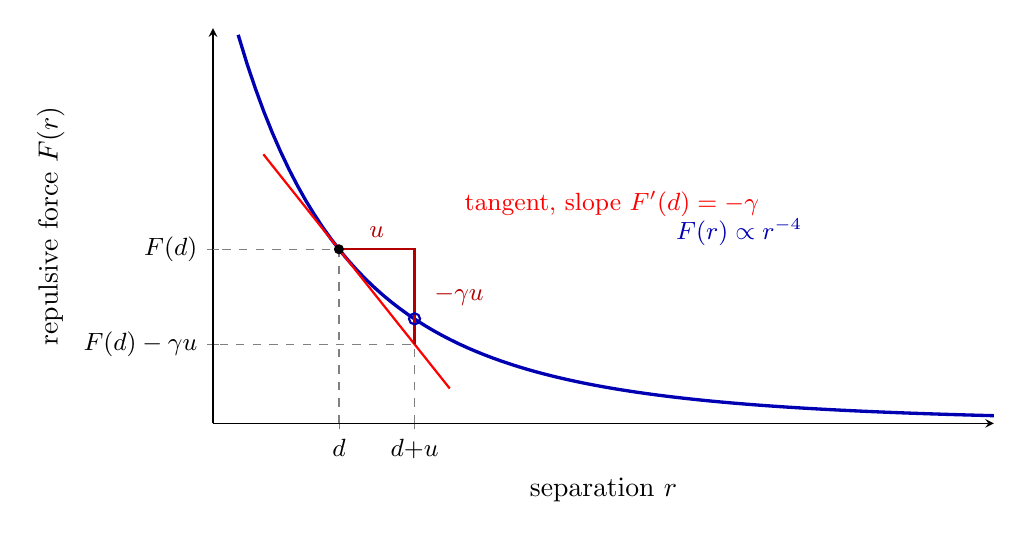
\begin{tikzpicture}
% d = 1.1, u = 0.15:  F(d)=1/1.1^4=0.683,  F'(d)=-4/1.1^5=-2.4837,
% tangent at d+u: 0.683-0.3726=0.310,  true F(1.25)=0.410
\begin{axis}[width=11.5cm,height=6.6cm,axis lines=left,
  xlabel={separation $r$},ylabel={repulsive force $F(r)$},
  xmin=0.85,xmax=2.4,ymin=0,ymax=1.55,
  xtick={1.1,1.25},xticklabels={$d$,$d{+}u$},xticklabel style={font=\small},
  ytick={0.683,0.310},yticklabels={$F(d)$,$F(d)-\gamma u$},yticklabel style={font=\small},
  clip=false]
\addplot[very thick,blue!70!black,domain=0.9:2.4,samples=90]{1/x^4};
\node[blue!70!black,anchor=west,font=\small] at (axis cs:1.75,0.75){$F(r)\propto r^{-4}$};
\addplot[red,thick,domain=0.95:1.32]{0.683-2.4837*(x-1.1)};
\node[red,anchor=west,font=\small] at (axis cs:1.33,0.86){tangent, slope $F'(d)=-\gamma$};
\draw[dashed,gray] (axis cs:1.1,0)--(axis cs:1.1,0.683)--(axis cs:0.85,0.683);
\draw[dashed,gray] (axis cs:1.25,0)--(axis cs:1.25,0.310)--(axis cs:0.85,0.310);
\draw[red!70!black,thick] (axis cs:1.1,0.683)--(axis cs:1.25,0.683)--(axis cs:1.25,0.310);
\node[red!70!black,above,font=\small] at (axis cs:1.175,0.69){$u$};
\node[red!70!black,anchor=west,font=\small] at (axis cs:1.27,0.50){$-\gamma u$};
\addplot[only marks,mark=*,mark size=1.6pt,black] coordinates{(1.1,0.683)};
\addplot[only marks,mark=o,mark size=2pt,blue!70!black,thick] coordinates{(1.25,0.410)};
\end{axis}
\end{tikzpicture}
\caption{Linearisation of the force law. Near the equilibrium separation $d$ the curve $F(r)$ is replaced by its tangent, whose slope is $-\gamma$. Increasing the separation by $u$ reduces the repulsion by $\gamma u$; decreasing it increases the repulsion by the same amount---the behaviour of a compressed spring of stiffness $\gamma$. The gap between the tangent and the true curve (open circle) is the error of the approximation; it grows with $u/d$ and is discussed in the evaluation.}
\end{figure}

\begin{figure}[H]
\centering
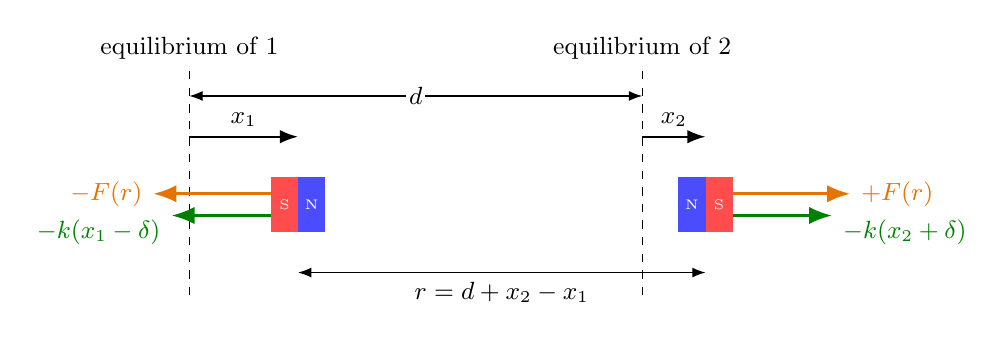
\begin{tikzpicture}[scale=1.15,>=Latex]
\draw[dashed] (0,-1.0)--(0,1.5); \draw[dashed] (5,-1.0)--(5,1.5);
\node[above,font=\small] at (0,1.5){equilibrium of 1}; \node[above,font=\small] at (5,1.5){equilibrium of 2};
\magnetSN{0.9}{-0.3}{0.6}{0.6}
\magnetNS{5.4}{-0.3}{0.6}{0.6}
\draw[->,thick] (0,0.75)--(1.2,0.75) node[midway,above,font=\small]{$x_1$};
\draw[->,thick] (5,0.75)--(5.7,0.75) node[midway,above,font=\small]{$x_2$};
\draw[<->] (1.2,-0.75)--(5.7,-0.75) node[midway,below,font=\small]{$r=d+x_2-x_1$};
\draw[<->] (0,1.2)--(5,1.2) node[midway,fill=white,inner sep=1pt,font=\small]{$d$};
\draw[->,very thick,orange!90!black] (0.9,0.12)--(-0.4,0.12) node[left,font=\small]{$-F(r)$};
\draw[->,very thick,green!50!black] (0.9,-0.12)--(-0.2,-0.12) node[left,font=\small,yshift=-6pt]{$-k(x_1-\delta)$};
\draw[->,very thick,orange!90!black] (6.0,0.12)--(7.3,0.12) node[right,font=\small]{$+F(r)$};
\draw[->,very thick,green!50!black] (6.0,-0.12)--(7.1,-0.12) node[right,font=\small,yshift=-6pt]{$-k(x_2+\delta)$};
\end{tikzpicture}
\caption{Free-body diagram of the two magnets (horizontal forces only, seen from above; orange: magnetic, green: elastic), both shown displaced to the right of their equilibrium positions. Each spring force is proportional to the displacement from that spring's \emph{unstressed} position ($+\delta$ for spring~1, $-\delta$ for spring~2, Figure~7). The magnetic force has magnitude $F(r)$ at the \emph{current} separation and pushes the magnets apart.}
\end{figure}

\begin{figure}[H]
\centering
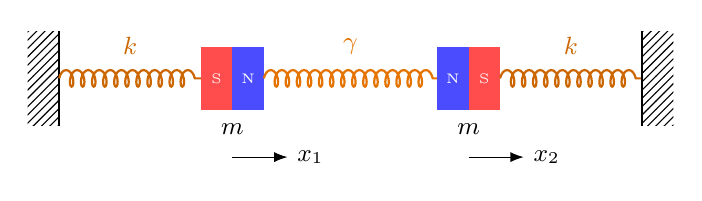
\begin{tikzpicture}[scale=1,>=Latex]
\fill[pattern=north east lines] (-0.4,-0.6) rectangle (0,0.6); \draw[thick](0,-0.6)--(0,0.6);
\draw[decorate,decoration={coil,aspect=0.5,segment length=4pt,amplitude=3pt},copper,thick] (0,0)--(1.8,0) node[midway,above=5pt,font=\small]{$k$};
\magnetSN{1.8}{-0.4}{0.8}{0.8}
\draw[decorate,decoration={coil,aspect=0.5,segment length=4pt,amplitude=3pt},orange!90!black,thick] (2.6,0)--(4.8,0) node[midway,above=5pt,font=\small]{$\gamma$};
\magnetNS{4.8}{-0.4}{0.8}{0.8}
\draw[decorate,decoration={coil,aspect=0.5,segment length=4pt,amplitude=3pt},copper,thick] (5.6,0)--(7.4,0) node[midway,above=5pt,font=\small]{$k$};
\fill[pattern=north east lines] (7.4,-0.6) rectangle (7.8,0.6); \draw[thick](7.4,-0.6)--(7.4,0.6);
\node[font=\small,below] at (2.2,-0.45){$m$}; \node[font=\small,below] at (5.2,-0.45){$m$};
\draw[->] (2.2,-1.0)--(2.9,-1.0) node[right,font=\small]{$x_1$};
\draw[->] (5.2,-1.0)--(5.9,-1.0) node[right,font=\small]{$x_2$};
\end{tikzpicture}
\caption{Mechanical equivalent of equations~(23): two equal masses $m$ on equal springs $k$ (copper: the leaf springs), coupled by a spring of stiffness $\gamma$ (orange: the magnetic repulsion). The picture is schematic; in the apparatus the coupling ``spring'' is the field between the magnets.}
\end{figure}

\begin{figure}[H]
\centering
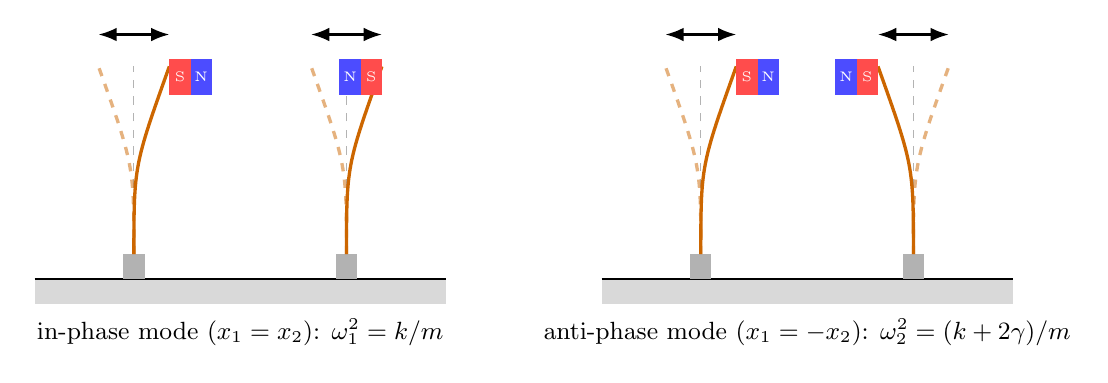
\begin{tikzpicture}[scale=0.9,>=Latex]
\foreach \dx/\lab/\sA/\sB in {0/{in-phase mode ($x_1=x_2$): $\omega_1^2=k/m$}/1/1, 8.0/{anti-phase mode ($x_1=-x_2$): $\omega_2^2=(k+2\gamma)/m$}/1/-1}{
 \begin{scope}[shift={(\dx,0)}]
  \fill[basegray] (-2.9,-0.35) rectangle (2.9,0); \draw[thick] (-2.9,0)--(2.9,0);
  \foreach \sx in {-1,1}{ \fill[clampgray] ({\sx*1.5-0.15},0) rectangle ({\sx*1.5+0.15},0.35); \draw[dashed,gray,opacity=0.6] ({\sx*1.5},0.35)--({\sx*1.5},3.0); }
  % the two extremes of the swing: solid and dashed (same one-control-point curves as in Section 1)
  \draw[very thick,copper] (-1.5,0.35) .. controls (-1.5,1.6) .. ({-1.5+0.5*\sA},3.0);
  \draw[very thick,copper,dashed,opacity=0.5] (-1.5,0.35) .. controls (-1.5,1.6) .. ({-1.5-0.5*\sA},3.0);
  \draw[very thick,copper] (1.5,0.35) .. controls (1.5,1.6) .. ({1.5+0.5*\sB},3.0);
  \draw[very thick,copper,dashed,opacity=0.5] (1.5,0.35) .. controls (1.5,1.6) .. ({1.5-0.5*\sB},3.0);
  % magnets on the inner faces at the solid extreme
  \magnetSN{-1.5+0.5*\sA}{2.6}{0.6}{0.5}
  \magnetNS{1.5+0.5*\sB-0.6}{2.6}{0.6}{0.5}
  \draw[<->,thick] ({-1.5-0.5},3.45)--({-1.5+0.5},3.45);
  \draw[<->,thick] ({1.5-0.5},3.45)--({1.5+0.5},3.45);
  \node[font=\small] at (0,-0.75) {\lab};
 \end{scope}
}
\end{tikzpicture}
\caption{The two normal modes (solid: one extreme of the swing; dashed: the other; magnets drawn at the solid extreme). Left, in-phase: the magnets keep their separation, the magnetic force never changes from its equilibrium value, and each spring oscillates as if alone, at $\omega_1=\sqrt{k/m}$. Right, anti-phase: when each magnet moves $a$ towards the other the separation shrinks by $2a$, so each magnet feels an extra restoring force $\gamma\cdot2a$ on top of $ka$; the effective stiffness is $k+2\gamma$.}
\end{figure}

\begin{figure}[H]
\centering
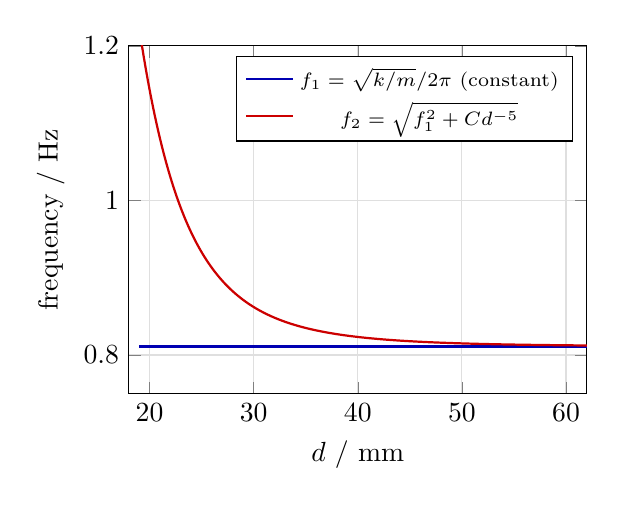
\begin{tikzpicture}
\begin{axis}[width=7.4cm,height=6cm,xlabel={$d$ / mm},ylabel={frequency / Hz},xmin=18,xmax=62,ymin=0.75,ymax=1.2,legend pos=north east,legend style={font=\scriptsize},grid=major,grid style={gray!25}]
\addplot[thick,blue!70!black,domain=19:62,samples=100]{0.811};
\addlegendentry{$f_1=\sqrt{k/m}/2\pi$ (constant)}
\addplot[thick,red!80!black,domain=19:62,samples=200]{sqrt(0.6577+2.08e6/x^5)};
\addlegendentry{$f_2=\sqrt{f_1^2+Cd^{-5}}$}
\end{axis}
\end{tikzpicture}\hfill
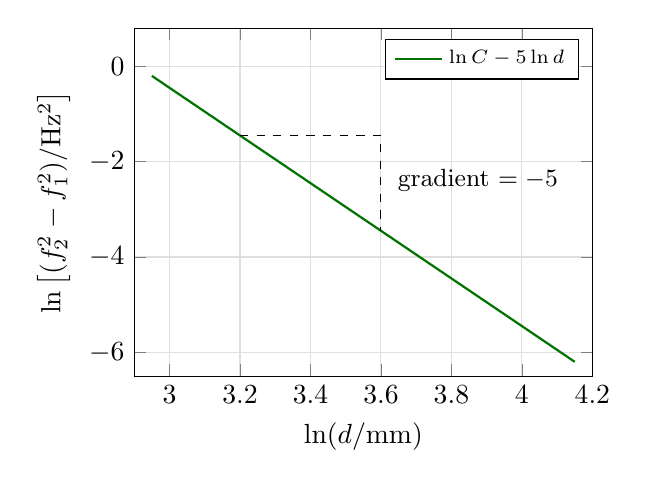
\begin{tikzpicture}
\begin{axis}[width=7.4cm,height=6cm,xlabel={$\ln(d/\mathrm{mm})$},ylabel={$\ln\big[(f_2^2-f_1^2)/\mathrm{Hz^2}\big]$},xmin=2.9,xmax=4.2,ymin=-6.5,ymax=0.8,grid=major,grid style={gray!25},legend pos=north east,legend style={font=\scriptsize}]
\addplot[thick,green!45!black,domain=2.95:4.15]{14.55-5*x};
\addlegendentry{$\ln C-5\ln d$}
\draw[dashed] (axis cs:3.2,-1.45)--(axis cs:3.6,-1.45)--(axis cs:3.6,-3.45);
\node[anchor=west] at (axis cs:3.62,-2.4){\small gradient $=-5$};
\end{axis}
\end{tikzpicture}
\caption{The prediction of the model, drawn with $f_1=0.811\un{Hz}$ and the value of $C$ obtained from the data. Left: $f_1$ is independent of $d$ while $f_2$ falls towards it. Right: the coupling term $f_2^2-f_1^2$ on logarithmic axes is a straight line of gradient exactly $-5$.}
\end{figure}

\begin{figure}[H]
\centering

\includegraphics[width=\textwidth]{fig_release.pdf}
\caption{The same system ($f_1=0.802$, $f_2=0.996\un{Hz}$; linear model, $A=8\un{mm}$) started in two ways; left: $x_1(t)$ with its envelope, right: its amplitude spectrum, with the predicted peak heights $\eta_0/2$ and $\xi_0/2$ marked. Top: idealised instantaneous release with $x_2(0)=0$---equal mode amplitudes, equal FFT peaks, beat minima at zero. Bottom: hold-and-release, $x_2(0)=A\gamma/(k+\gamma)=1.7\un{mm}$---peak ratio $(f_1/f_2)^2=0.65$ and beat minima of $1.7\un{mm}$. The peak \emph{positions} are identical in both cases. (Generated by \texttt{make\_fig\_release.py}.)}
\end{figure}

\begin{figure}[H]
\centering
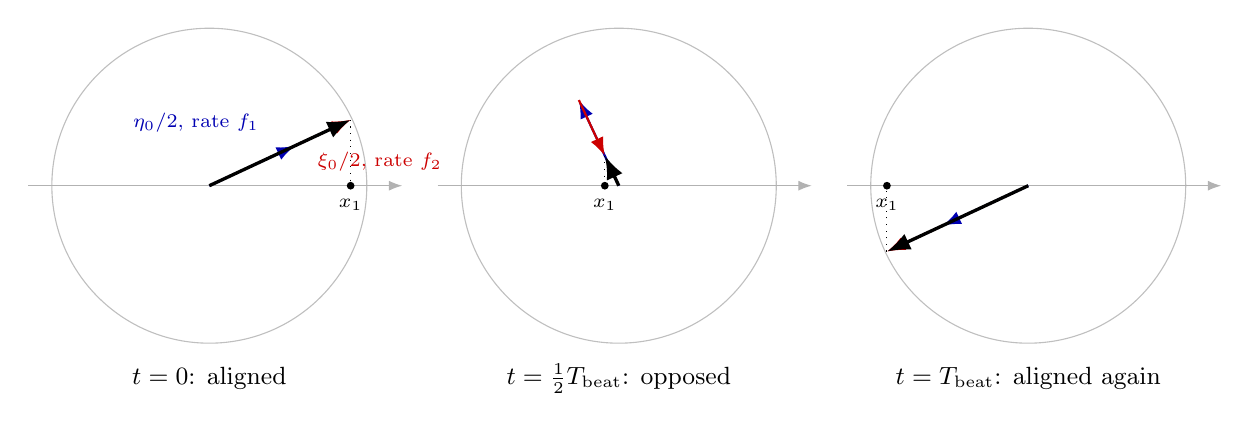
\begin{tikzpicture}[scale=1.0,>=Latex]
\foreach \dx/\ta/\tb/\capA in {0/25/25/{$t=0$: aligned},
                               5.2/115/295/{$t=\tfrac12T_{\rm beat}$: opposed},
                               10.4/205/205/{$t=T_{\rm beat}$: aligned again}}{
 \begin{scope}[shift={(\dx,0)}]
  \draw[gray!50] (0,0) circle (2.0);
  \draw[gray!60,->] (-2.3,0)--(2.45,0);
  \draw[->,thick,blue!70!black] (0,0)--(\ta:1.2) coordinate (p);
  \draw[->,thick,red!80!black] (p)--++(\tb:0.78) coordinate (q);
  \draw[->,very thick,black] (0,0)--(q);
  \draw[dotted] (q)--(q|-0,0);
  \fill (q|-0,0) circle (1.4pt);
  \node[below,font=\scriptsize] at ($(q|-0,0)+(0,-0.05)$) {$x_1$};
  \node[font=\small] at (0,-2.45) {\capA};
 \end{scope}
}
\node[blue!70!black,font=\scriptsize,anchor=south east] at (0.75,0.55) {$\eta_0/2$, rate $f_1$};
\node[red!80!black,font=\scriptsize,anchor=north west] at (1.25,0.55) {$\xi_0/2$, rate $f_2$};
\end{tikzpicture}
\caption{Beats as rotating arrows (phasors). Blue: length $\eta_0/2$, turning at $f_1$ revolutions per second. Red, drawn head-to-tail: length $\xi_0/2$, turning at $f_2$. Black: their sum; $x_1$ is its horizontal projection. The relative angle grows by one full turn every $1/(f_2-f_1)$ seconds, so the length of the black arrow---the amplitude of the fast oscillation---swings between $(\eta_0+\xi_0)/2$ and $|\eta_0-\xi_0|/2$ with exactly that period. Drawn for $\xi_0/\eta_0=0.65$, the hold-and-release case: the amplitude never falls to zero.}
\end{figure}

\begin{figure}[H]
\centering
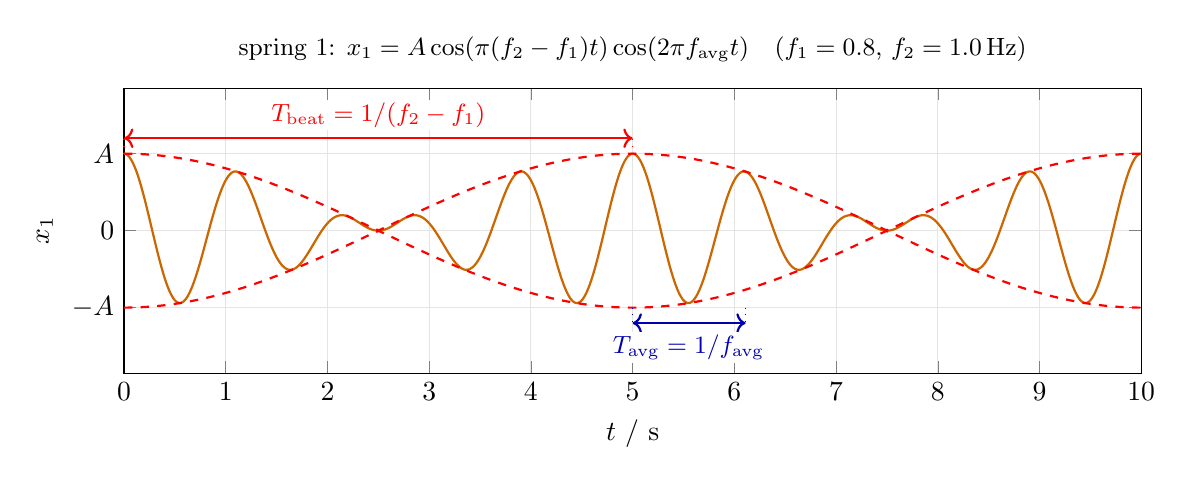
\begin{tikzpicture}
\begin{axis}[width=14.5cm,height=5.2cm,xlabel={$t$ / s},ylabel={$x_1$},xmin=0,xmax=10,ymin=-1.85,ymax=1.85,ytick={-1,0,1},yticklabels={$-A$,$0$,$A$},grid=major,grid style={gray!20},clip=false,title={\small spring 1: $x_1=A\cos(\pi(f_2-f_1)t)\cos(2\pi f_{\rm avg}t)$\quad ($f_1=0.8$, $f_2=1.0\un{Hz}$)}]
\addplot[thick,copper,domain=0:10,samples=700]{cos(deg(0.2*pi*x))*cos(deg(1.8*pi*x))};
\addplot[thick,red,dashed,domain=0:10,samples=300]{abs(cos(deg(0.2*pi*x)))};
\addplot[thick,red,dashed,domain=0:10,samples=300]{-abs(cos(deg(0.2*pi*x)))};
\draw[dotted,red] (axis cs:0,1)--(axis cs:0,1.25); \draw[dotted,red] (axis cs:5,1)--(axis cs:5,1.25);
\draw[<->,thick,red] (axis cs:0,1.2)--(axis cs:5,1.2);
\node[red,fill=white,inner sep=1pt] at (axis cs:2.5,1.5){\small $T_{\rm beat}=1/(f_2-f_1)$};
\draw[dotted,blue!70!black] (axis cs:5,-1)--(axis cs:5,-1.25); \draw[dotted,blue!70!black] (axis cs:6.111,-1)--(axis cs:6.111,-1.25);
\draw[<->,thick,blue!70!black] (axis cs:5,-1.2)--(axis cs:6.111,-1.2);
\node[blue!70!black,fill=white,inner sep=1pt] at (axis cs:5.55,-1.52){\small $T_{\rm avg}=1/f_{\rm avg}$};
\end{axis}
\end{tikzpicture}\\
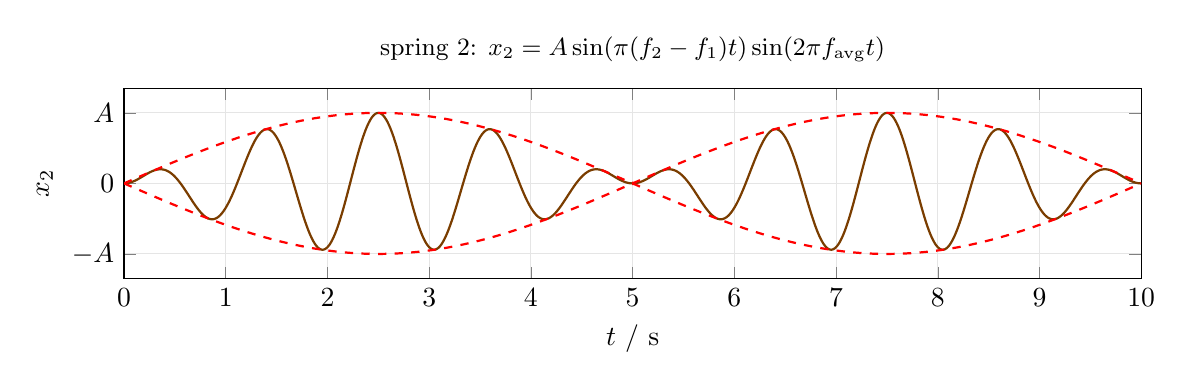
\begin{tikzpicture}
\begin{axis}[width=14.5cm,height=4.0cm,xlabel={$t$ / s},ylabel={$x_2$},xmin=0,xmax=10,ymin=-1.35,ymax=1.35,ytick={-1,0,1},yticklabels={$-A$,$0$,$A$},grid=major,grid style={gray!20},title={\small spring 2: $x_2=A\sin(\pi(f_2-f_1)t)\sin(2\pi f_{\rm avg}t)$}]
\addplot[thick,copper!60!black,domain=0:10,samples=700]{sin(deg(0.2*pi*x))*sin(deg(1.8*pi*x))};
\addplot[thick,red,dashed,domain=0:10,samples=300]{abs(sin(deg(0.2*pi*x)))};
\addplot[thick,red,dashed,domain=0:10,samples=300]{-abs(sin(deg(0.2*pi*x)))};
\end{axis}
\end{tikzpicture}
\caption{Beats for equal mode amplitudes. Top: the released spring and its envelope (red dashed); the swellings recur every $T_{\rm beat}=1/(f_2-f_1)$, and the fast oscillation has period $1/f_{\rm avg}$. Bottom: spring~2 carries the same two frequencies with the anti-phase term reversed, $x_2=\frac A2(\cos\omega_1t-\cos\omega_2t)=A\sin(\pi(f_2-f_1)t)\sin(2\pi f_{\rm avg}t)$; its envelope is a quarter of a beat behind, so it swings most when spring~1 is momentarily still. This is the energy transfer between the springs.}
\end{figure}

\end{document}
